\section{Bilanciamento del bianco} \label{sec:whitebalance}
Il modo in cui l'occhio umano e un sensore vedono la luce non è lo stesso.

L'occhio umano, entro certi limiti, fa delle compensazioni. Una carta da gioco la vediamo bianca a tutte le ore del giorno, nonostante la luce cambi molto, passando da tonalità molto fredde, sul blu, del mattino e delle notte, alle tonalità neutre del mezzogiorno, e se siamo fortunati a tonalità molto calde, sull'arancione e sul rosso all'alba e al tramonto.
È il motivo per cui, se fissiamo una mela rossa su un foglio bianco, e poi distogliamo lo sguardo, vedremo per un po' una mela verde; è il nostro cervello che cerca di compensare i colori.
Questo effetto si chiama \textbf{costanza percettiva}.

I sensori non fanno niente di tutto ciò: se osserviamo una scena calda le fotocamera vedrà tutti i colori tinti di rosso e arancione, senza cerca di fare alcuna compensazione.
Sarà compito di chi fotografa dire alla fotocamera come compensare la luce.

\subsection{Scala Kelvin} \label{subsec:scalakelvin}
Per poter valutare la tonalità della luce, o \textit{temperatura}, Lord William Thomson ha inventato nel 1848 la \textbf{Scala Kelvin} (mostrata in figura~\ref{fig:scala_kelvin}).
L'unità di misura usata per determinare la temperatura della luce è il \textit{Kelvin}, in breve \text{K}.

Parte dai $1\,000K$ per la luce più calda e arriva ai $16\,000K$ per la luce più fredda. Le scale spesso mostrano l'intervallo $1\,800K - 10\,000K$, più che sufficiente per molte situazioni.

La luce neutra, bianca, ha un valore di $5\,500K$. È la temperatura usata dai flash ed è, all'incirca, la temperatura della luce solare a mezzogiorno.

\begin{figure}[h]
    \centering
    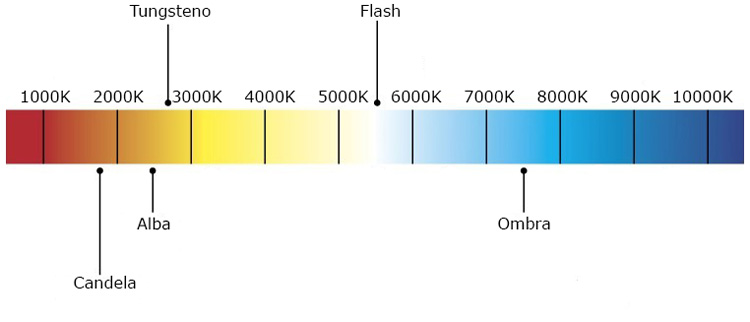
\includegraphics[width=\textwidth]{Kelvin.jpg}
    \caption{Scala Kelvin}
    \label{fig:scala_kelvin}
\end{figure}


\subsection{Bilanciamento sulle fotocamere} \label{subsec:bilaciamentofotocamere}
Le fotocamere permettono di bilanciare la temperatura della luce, con dei valori predefiniti (il più delle volte sufficienti) o con valori personalizzati.

L'impostazione di default è \textbf{AWB - Auto White Balance}, in questo caso non dobbiamo occuparcene noi ma è la fotocamera a valutare la situazione e ad impostare il bilanciamento del bianco.
I primi tempi è l'opzione più comoda, così il fotografo neofita non è gravato da una cosa in più a cui pensare; inoltre funziona solitamente molto bene, si possono ottenere quindi risultati più che accettabili.

I bilanciamenti solitamente disponibili sulle macchinette sono riportati nella Tabella~\ref{table:white_balance}.
\begin{table}[h]
    \centering
    \begin{tabular}{|l|l|} 
    \hline
    Luce diurna              & $5200K\sim$\\ 
    \hline
    Ombra                    & $7000K\sim$\\ 
    \hline
    Nuvoloso                 & $6000K\sim$\\ 
    \hline
    Tungsteno                & $3200K\sim$\\ 
    \hline
    Luce bianca fluorescente & $4000K\sim$\\ 
    \hline
    Flash                    &                           \\ 
    \hline
    Personalizzato           &                           \\
    \hline
    \end{tabular}
    \caption{Bilanciamento del bianco}
    \label{table:white_balance}
\end{table}

\nb Sono valori approssimativi, per questo l'aggiunta della tilde (i.e. $\sim$).

Il valore che impostiamo non è la temperatura che il sensore cercherà di emulatore. Indica la temperatura a cui ci troviamo, e quindi il sensore aggiungerà della luce opposta per bilanciare e cercare di far appare il bianco come effettivamente bianco (i.e. \textit{bilanciamento del bianco}).

Se ad esempio impostiamo \textit{ombra}, significa che ci troviamo in una situazione di luce molto fredda, e la macchinetta cercherà di compensare con colori caldi.

È un problema se il bilanciamento del bianco è sbagliato? Se scattiamo in raw (vedi \nameref{sec:rawjpeg}) no, il bilanciamento si può sistemare in un secondo momento in post produzione senza perdere qualità.
Se invece la foto è scattata in jpg potrebbe esserci qualche piccola perdita di dettagli, ma se le correzioni sono leggere non è un problema.

È comunque una buona idea cercare di impostare correttamente il bilanciamento del bianco già nel momento in cui si scatta, sia per avere subito un'idea di come la foto esce fuori (più sono le modifiche da fare dopo più bisogna essere bravi ad immaginare in anticipo il risultato), sia per perdere meno tempo in post produzione.